\documentclass[a4paper,12pt]{article}
\usepackage{xeCJK}          % 中文支持
\usepackage{fontspec}       % 英文/数学字体
\usepackage{amsmath, amssymb} % 数学公式
\usepackage{graphicx}       % 插入图片
\usepackage{hyperref}       % 目录超链接
\usepackage{geometry}       % 页面布局
\usepackage{bm}             % 粗体
\usepackage{xcolor}         % 颜色
\usepackage{tabularx}       % 表格环境
\usepackage{tikz}           % TikZ 绘制主对角线斜线
\usepackage{tcolorbox}
\usepackage{xstring}
\usepackage{pgfplots}
\usepackage{enumitem}
\usepackage{pifont}
\usepackage{ulem}
\usepackage{mathtools}
\usepackage{dsfont}
\usepackage{extarrows}
\usepackage{amssymb}
\usepgfplotslibrary{fillbetween}
\pgfplotsset{compat=1.18}
\geometry{left=3cm,right=3cm,top=3cm,bottom=3cm}

\definecolor{customgreen}{rgb}{0.2,0.6,0.3}
\newcommand{\gmath}[1]{\textcolor{customgreen}{#1}}

% 经典
\definecolor{classicgreen}{rgb}{0.1,0.5,0.3}
\newtcbox{\classic}{
    on line,
    colback=classicgreen!10,
    colframe=classicgreen,
    boxrule=0.8pt,
    arc=3pt,
    boxsep=1pt,
    left=4pt,
    right=4pt,
    top=2pt,
    bottom=2pt
}

% 抽离颜色和尺寸参数
\newcommand{\analysisTitleColor}{green!50!black}
\newcommand{\analysisBackColor}{white}
\newcommand{\analysisBoxRule}{0.8pt}
\newcommand{\analysisArc}{3pt}
\newcommand{\analysisPadding}{6pt}

% 定义 tcolorbox
\newtcolorbox{analysisbox}[1][]{
    title=\IfStrEq{#1}{}{\textbf{解析}}{#1}, % 如果传参为空则使用“解析”
    colback=\analysisBackColor,
    colframe=\analysisTitleColor,
    boxrule=\analysisBoxRule,
    arc=\analysisArc,
    left=\analysisPadding,
    right=\analysisPadding,
    top=4pt,
    bottom=4pt
}

\newlist{circlenum}{enumerate}{1}
\setlist[circlenum]{
    label=\ding{\numexpr171+\arabic*},
    leftmargin=2.2em,
    itemsep=0.6em,      % item 之间的距离（主要）
    topsep=0.6em,       % 列表与上下正文的距离
    parsep=0.3em,       % item 内段落的间距
    partopsep=0.3em     % 列表前后额外间距
}

\newcommand{\blueuline}[1]{{\color{blue}\uline{\color{black}{#1}}}}

% =========================
% 字体设置
% =========================
\setmainfont{Times New Roman}
\setsansfont{Helvetica Neue}
\setmonofont{Menlo}
\setCJKmainfont{PingFang SC}

% =========================
% 图形路径（可调整）
% =========================
\graphicspath{{./assets/}}

% =========================
% 文档开始
% =========================
\begin{document}

%    \title{Template}
%    \author{Bowen}
%    \date{\today}
%    \maketitle
%    \tableofcontents
%    \newpage


% =========================

    \section{一元函数积分学的应用 - 几何应用}

    \subsection{用定积分表达和计算平面图形的面积}

    \begin{enumerate}
        \item 曲线$y = y_1(x)$与$y = y_2(x)$及$x = a, x = b(a < b)$所围成的平面图形的面积
        \[
            S = \int_a^b |y_1(x) - y_2(x)|\,\mathrm{d}x
        \]
        \item 曲线$r = r_1(\theta)$与$r = r_2(\theta)$与两射线$\theta = \alpha$与$\theta = \beta(0 < \beta - \alpha \leq 2\pi)$所围成的曲边扇形的面积
        \[
            S = \frac{1}{2}\int_{\alpha}^{\beta} |r_1^2(\theta) - r_2^2(\theta)|\,\mathrm{d}\theta
        \]
        \item 参数方程下面积公式的本质：直接坐标系下的面积公式的\textbf{\blueuline{换元法形式}}
        \[
            S = \int_a^b f(x)\,\mathrm{d}x  \xlongequal{x = x(t)} \int_{x^{-1}(a)}^{x^{-1}(b)} f[x(t)]d[x(t)] = \int_{x^{-1}(a)}^{x^{-1}(b)} y(t)x'(t)\,\mathrm{d}t
        \]
    \end{enumerate}

    \subsection{用定积分表达和计算旋转体的体积}

    \begin{enumerate}
        \item 曲线$y = y(x)$与$x = a, x = b(a < b)$及$x$轴围成的曲边梯形绕$x$轴旋转一周所得到的的旋转体的体积
        \[
            V_x = \int_a^b \pi y^2(x)\,\mathrm{d}x
        \]
        \item 曲线$y = y(x)$与$x = a, x = b(0 \leq a < b)$及$x$轴围成的曲边梯形绕$y$轴旋转一周所得到的的旋转体的体积
        \[
            V_y = 2\pi\int_a^b x|y(x)|\,\mathrm{d}x
        \]
        \item 平面曲线绕定直线旋转

        平面曲线$L: y = f(x), a \leq x \leq y$，且$f(x)$可导

        定直线$L_0: Ax + By + C = 0$，且过$L_0$的任一条垂线与$L${\blueuline{至多有一个交点}}，则$L$绕$L_0$旋转一周所得旋转体的体积
        \[
                {\color{red}{\bigstar}}V = \frac{\pi}{(A^2 + B^2)^{\frac{3}{2}}}\int_a^b [Ax + Bf(x) + C]^{\color{red}{2}}|Af'(x) - B|\,\mathrm{d}x
        \]
    \end{enumerate}

    \subsection{用定积分表达和计算函数的平均值}

    设$x \in [a, b]$，函数$y(x)$在$[a, b]$上的平均值为$\bar{y} = \displaystyle\frac{1}{b - a}\int_a^b y(x)\,\mathrm{d}x \Rightarrow \bar{y} = y(\xi), \xi \in [a, b]$

    \subsection{平面上的曲边梯形的形心坐标公式}

    设平面区域$D = \{(x, y) \mid 0 \le y \le f(x),\ a \le x \le b\}$，其中 $y = f(x)$ 在 $[a,b]$ 上连续。则区域 $D$ 的形心坐标 $\bar{x},\,\bar{y}$ 为
    \[
        \begin{aligned}
            \bar{x}
            &=
            \frac{\displaystyle\int_a^b x f(x)\,\mathrm{d}x}
            {\displaystyle\int_a^b f(x)\,\mathrm{d}x},
            \\[8pt]
            \bar{y}
            &=
            \frac{\displaystyle\frac{1}{2}\int_a^b f^2(x)\,\mathrm{d}x}
            {\displaystyle\int_a^b f(x)\,\mathrm{d}x}.
        \end{aligned}
    \]

    \subsection{平面曲线的弧长}

    \begin{enumerate}
        \item 若平面光滑曲线由直角坐标方程$y = y(x)(a \leq x \leq b)$给出，则$s = \displaystyle\int_a^b \sqrt {1 + [y'(x)]^2}\,\mathrm{d}x$
        \item 若平面光滑曲线由参数方程$\begin{cases}
                                           x = x(t), \\
                                           y = y(x)
        \end{cases}(\alpha \leq t \leq \beta)$给出，则$s = \displaystyle\int_{\alpha}^{\beta} \sqrt {[x'(t)]^2 + [y'(t)]^2}\,\mathrm{d}t$
        \item 若平面光滑曲线由极坐标方程$r = r(\theta)(\alpha \leq \theta \leq \beta)$给出，则$s = \displaystyle\int_{\alpha}^{\beta} \sqrt {[r(\theta)]^2 + [r'(\theta)]^2}\,\mathrm{d}\theta$
    \end{enumerate}

    \subsection{旋转曲面的面积（侧面积）}

    {\color{customgreen}{在弧长公式基础上多乘了$2\pi|y(x)|$}}

    \begin{enumerate}
        \item 曲线$L: y = f(x)(a \leq x \leq b)$绕$x$轴旋转一周所得旋转曲面的面积
        \[
            S = 2\pi\int_a^b |y|\sqrt {1 + (y'_x)^2}\,\mathrm{d}x
        \]
        \item 曲线$L: \begin{cases}
                          x = x(t), \\
                          y = y(t)
        \end{cases}(\alpha \leq t \leq \beta, x'(t) \neq 0)$绕$x$轴旋转一周所得旋转曲面的面积
        \[
            S = 2\pi\int_{\alpha}^{\beta} |y(t)|\sqrt {(x_t')^2 + (y_t')^2}\,\mathrm{d}t
        \]
        \item 曲线$L: r = r(\theta)(\alpha \leq \theta \leq \beta)$绕$x$轴旋转一周所得旋转曲面的面积
        \[
            S = 2\pi\int_{\alpha}^{\beta} |r(\theta)\sin \theta|\sqrt {[r(\theta)]^2 + [r'(\theta)]^2}\,\mathrm{d}\theta
        \]
    \end{enumerate}

    \subsection{平行截面面积为已知的立体体积}

    在区间$[a, b]$上，垂直于$x$轴的平面截立体$\Omega$所得到的的截面面积为$x$的连续函数$A(x)$，取体积微元: $dV = A(x)\,\mathrm{d}x$，则$\Omega$的体积为
    \[
        V = \int_a^b A(x)\,\mathrm{d}x
    \]

    \subsection{基础概念}

    \begin{enumerate}
    \end{enumerate}

    \subsection{结论}

    \begin{enumerate}
        \item 摆线（平摆线）\begin{cases}
                              x = a(t - \sin t), \\
                              y = a(1 - \cos t)
        \end{cases}$(a > 0)$的一拱与$x$轴所围平面图形的面积是$3a^2\pi$
        \begin{center}
            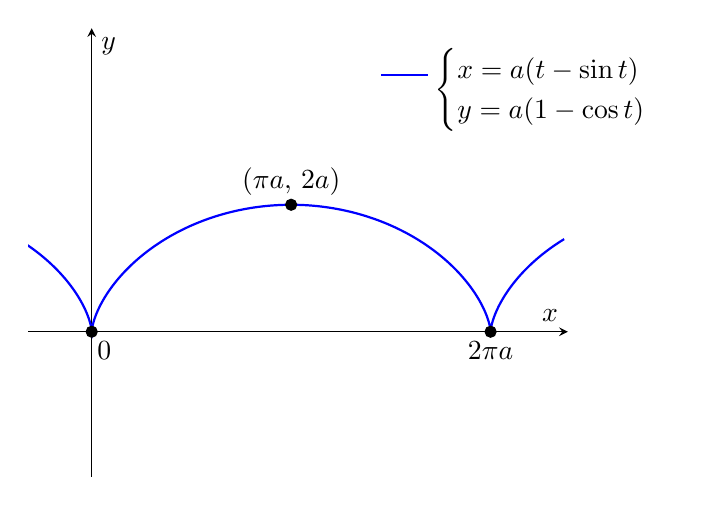
\begin{tikzpicture}
                \begin{axis}
                    [
                    axis equal,
                    axis lines=middle,
                    xmin=-1, xmax=7.5,
                    ymin=-0.5, ymax=3,
                    samples=400,
                    domain=-2.0472:8.33038,
                    xlabel={$x$},
                    ylabel={$y$},
                    xtick=\empty,
                    ytick=\empty,
                    legend style={
                        at={(0.02,0.98)},
                        anchor=north west,
                        xshift=120pt,
                        yshift=0pt,
                        draw=none
                    }
                    ]

% 摆线 (a=1)
                    \addplot[
                        thick,
                        blue
                    ]
                    ({x - sin(deg(x))},
                        {1 - cos(deg(x))});

                    \addlegendentry{
                        $\begin{cases}
                             x=a(t-\sin t)\\
                             y=a(1-\cos t)
                        \end{cases}$
                    }

% x轴交点
                    \addplot[only marks] coordinates {(0,0)};
                    \addplot[only marks] coordinates {(6.28318,0)};

                    \node at (axis cs:0.2,-0.3) {$0$};
                    \node[below] at (axis cs:6.28318,0) {$2\pi a$};

% 最高点
                    \addplot[only marks] coordinates {(3.14159,2)};
                    \node[above] at (axis cs:3.14159,2)
                        {$(\pi a,\,2a)$};

                \end{axis}
            \end{tikzpicture}
        \end{center}
        \item 伯努利双纽线$r^2 = a^2\cos 2\theta$围成的图形的面积是$a^2$

        \begin{center}
            \begin{tikzpicture}
                \begin{axis}
                    [
                    axis equal,
                    axis lines=middle,
                    xlabel={$x$},
                    ylabel={$y$},
                    enlarge x limits=0.3,
                    domain=-45:45,
                    samples=400,
                    xtick=\empty,
                    ytick=\empty,
                    legend style={
                        at={(0.02,0.98)},
                        anchor=north west,
                        xshift=120pt,
                        yshift=0pt,
                        draw=none
                    }
                    ]
                    \addplot[
                        blue,
                        thick
                    ]
                    ({cos(x)*sqrt(cos(2*x))},
                        {sin(x)*sqrt(cos(2*x))});

                    \addplot[
                        blue,
                        thick
                    ]
                    ({-cos(x)*sqrt(cos(2*x))},
                        {-sin(x)*sqrt(cos(2*x))});

                    \addlegendentry{$r^2 = a^2 \cos(2\theta)$}
                \end{axis}
            \end{tikzpicture}
        \end{center}
    \end{enumerate}

    \subsection{定理}

    \begin{enumerate}
    \end{enumerate}

    \subsection{运算}

    \begin{enumerate}

    \end{enumerate}

    \subsection{公式}

    \begin{enumerate}

        \item 等比公式前$n$项和: $S_n = \displaystyle\frac{a(1-r^n)}{1-r} = \displaystyle\frac{ar^n - a}{r - 1}, \quad r \ne 1 $
    \end{enumerate}

    \subsection{方法总结}

    \begin{enumerate}
        \item 注意自变量$x$的取值范围。\emph{e.g.} $y = e^{-\frac{x}{2}}\sqrt {\sin x}$在$[0, 2\pi]$部分$\Rightarrow \sqrt {\sin x} \Rightarrow \sin x \geq 0 \Rightarrow x \in [0, \pi]$

    \end{enumerate}

    \subsection{条件转换思路}

    \begin{enumerate}

    \end{enumerate}

    \subsection{理解}

    \begin{enumerate}
    \end{enumerate}

\end{document}
